\documentclass[11pt,a4paper]{article}
\usepackage[utf8]{inputenc}
\usepackage[T1]{fontenc}
\usepackage{amsmath,amssymb,amsthm}
\usepackage{booktabs}
\usepackage{graphicx}
\usepackage{subcaption}
\usepackage{microtype}
\usepackage{xcolor}
\usepackage{float}
\usepackage[margin=1.1in]{geometry}
\usepackage[colorlinks=true,linkcolor=blue!60!black,citecolor=blue!60!black,urlcolor=blue!60!black]{hyperref}
\graphicspath{{figures/}}

\newtheorem{theorem}{Theorem}[section]
\newtheorem{proposition}[theorem]{Proposition}
\newtheorem{lemma}[theorem]{Lemma}
\newtheorem{corollary}[theorem]{Corollary}
\theoremstyle{definition}
\newtheorem{definition}[theorem]{Definition}
\theoremstyle{remark}
\newtheorem{remark}[theorem]{Remark}

\newcommand{\R}{\mathbb{R}}
\newcommand{\Z}{\mathbb{Z}}
\newcommand{\Q}{\mathbb{Q}}
\newcommand{\E}{\mathbb{E}}
\newcommand{\TV}{\operatorname{TV}}
\newcommand{\frc}{\operatorname{frac}}
\DeclareMathOperator{\dist}{dist}
\DeclareMathOperator{\codim}{codim}

\title{Apparent Complexity of Quantized Diffusion:\\
  Contour Maps, Aliasing and Moir\'e}
\author{Miguel E.~P\'erez Ibarra\thanks{Affiliation and e-mail. (Placeholder.)}
  \and Jaziel Flores Rodr\'iguez\thanks{Affiliation and e-mail. (Placeholder.)}}
\date{\today\\[4pt]\small Code and figures: \url{https://github.com/MiguelPerezI/heat-parity-ca}}

\begin{document}
\maketitle

\begin{abstract}
Colouring the cells of a finite-difference heat simulation by the
parity of $\lfloor q\,u\rfloor$ produces black-and-white frames whose
apparent complexity rises from nothing, peaks in a lattice of symmetric
concentric islands, and dies. We show that these frames are the contour
map of the temperature at spacing $1/q$ with alternating fill, that the
rise is aliasing, and that the islands are the replicated centres of an
undersampled Fresnel zone plate. Three elementary results make this
exact: the band count and the total variation are nonincreasing under
Neumann heat flow on a box; the phase-averaged perimeter of the sampled
pattern equals a sum over grid edges of a triangle wave of the edge
jump, $\sum_e \dist(q|\Delta_e u|,2\Z)$, and the discrete total
variation is nonincreasing, so every increase of the perimeter is
produced by edges whose jump exceeds one quantum; and the block entropy
of the pattern has two non-commuting limits, $0$ as the grid is refined
and maximal as the quantum is refined. The pictures are therefore
not a new cellular automaton but a clean example of how complexity
measures of a thresholded field report the sampling rather than the
dynamics; we close with a remark on why this matters for proposed laws of
increasing functional information.
\end{abstract}

\section{The observation}\label{sec:obs}

The two-dimensional heat equation $u_t=\kappa\Delta u$ was integrated on
a $64\times64$ grid with an explicit scheme, starting from a hot square
($u=100$ on a $24\times24$ block, $0$ elsewhere), and displayed as a
height field in which each facet is coloured white or black according to
the parity of $\lfloor 10\,u\rfloor$. The frames (Figure~\ref{fig:frames})
begin uniformly black, erupt into a fine noise-like texture around the
square, organize into a square-symmetric lattice of concentric islands,
and finally fade to a few rings and then to a single colour. The
sequence looks like a cellular automaton with a rich transient, and the
islands look like eddies. Neither is the case, and the point of this
note is to say precisely what they are.

\begin{figure}[ht]
\centering
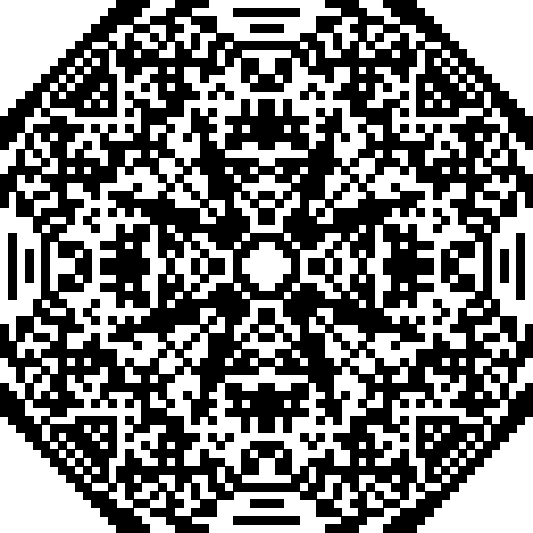
\includegraphics[width=0.3\textwidth]{parity_k150.pdf}\hfill
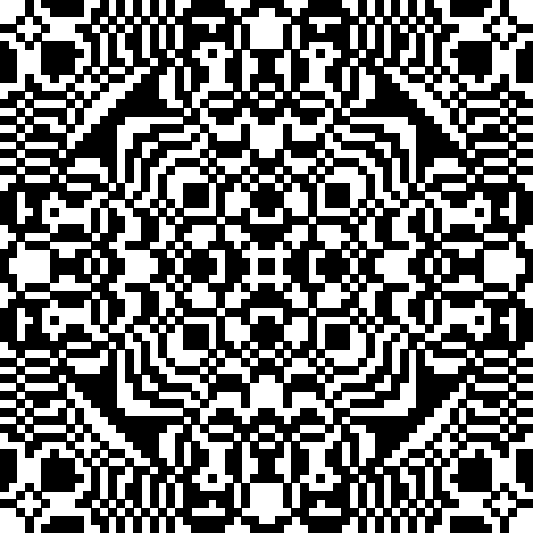
\includegraphics[width=0.3\textwidth]{parity_k1000.pdf}\hfill
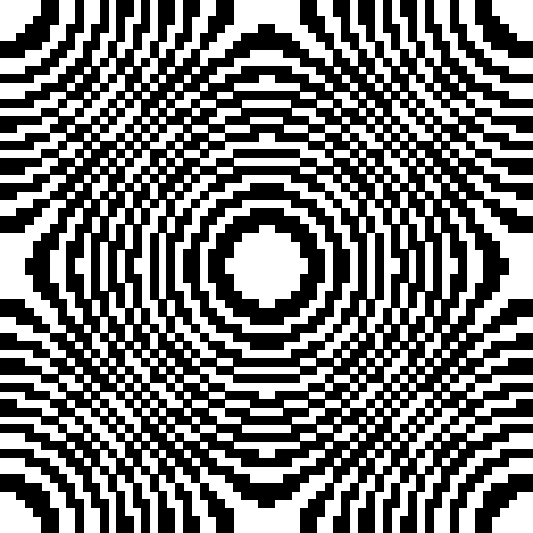
\includegraphics[width=0.3\textwidth]{parity_k2000.pdf}
\caption{Parity of $\lfloor 10u\rfloor$ on the $64\times64$ grid at
steps $150$, $1000$ and $2000$ of the explicit scheme with
$\Delta t=2\cdot10^{-4}$, $\kappa=0.2$, reflecting walls. The field has a
single maximum throughout.}
\label{fig:frames}
\end{figure}

Throughout, $\Omega=(0,L)^n$, $u$ solves $u_t=\kappa\Delta u$ with
homogeneous Neumann data, $q>0$ is the quantization frequency (quantum
$1/q$), $\theta\in[0,1)$ is a phase, and the \emph{pattern} is
\begin{equation}\label{eq:pattern}
  b_\theta(x,t)=\lfloor q\,u(x,t)+\theta\rfloor \bmod 2 .
\end{equation}
The grid version samples $u$ at the $N^n$ nodes of the explicit scheme
with reflected ghost values (the ternary-cube rule of \cite{TernaryCube} with zero flux), under
$\sum_m r_m\le\frac12$. We write $E$ for the set of grid edges and
$\Delta_eu$ for the jump of $u$ across the edge $e$.

So \eqref{eq:pattern} is the contour map of $u$ with isotherms at the
levels $(k-\theta)/q$ and alternating fill. The pattern is an
\emph{observable} of $u$, not a state: two fields with the same pattern
evolve to different patterns, so no local rule on black and white cells
reproduces the frames, and by the usual definition (a map on
configurations over a finite alphabet given by a local rule
\cite{MOW}) this is not a cellular automaton.

\section{What is monotone in the continuum}\label{sec:cont}

\begin{theorem}\label{thm:cont}
Let $u$ solve the Neumann heat equation on the box $\Omega$.
\begin{enumerate}
\item The band count $B_q(t)=\#\{k:(k-\theta)/q\in[\min u(\cdot,t),\max u(\cdot,t)]\}$ is nonincreasing for every $\theta$.
\item The total variation $\TV(t)=\int_\Omega|\nabla u(x,t)|\,dx$ is nonincreasing.
\item The phase-averaged total isotherm length equals the total variation exactly:
\begin{equation}\label{eq:coarea}
  \int_0^1\sum_{k\in\Z}\mathcal H^{n-1}\bigl(\{u(\cdot,t)=(k-\theta)/q\}\bigr)\,d\theta
  \;=\; q\,\TV(t),
\end{equation}
and is therefore nonincreasing.
\end{enumerate}
\end{theorem}

\begin{proof}
(1) is the maximum principle \cite{Evans}: $\max u$ is nonincreasing and $\min u$
nondecreasing. (2) Reflect $u$ evenly across every face of the box; the
result $\tilde u$ is a $2L$-periodic solution of the heat equation on the
torus $\mathbb T=(\R/2L\Z)^n$, smooth for $t>0$. Each component
$\partial_m\tilde u$ is again a periodic heat solution, so
$\nabla\tilde u(t)=K_{t-s}*\nabla\tilde u(s)$ for $t>s$, where $K$ is the
periodic heat kernel, $K\ge0$, $\int K=1$. Convexity of the Euclidean
norm gives $|\nabla\tilde u(t)|\le K_{t-s}*|\nabla\tilde u(s)|$
pointwise; integrating over $\mathbb T$ and dividing by $2^n$ gives
$\TV(t)\le\TV(s)$. (3) By the coarea formula,
$\int_\Omega|\nabla u|=\int_\R\mathcal H^{n-1}(\{u=s\})\,ds$; the left
side of \eqref{eq:coarea} is $\int_\R\mathcal H^{n-1}(\{u=s\})\,q\,ds$
after the substitution $s=(k-\theta)/q$, $\theta\in[0,1)$, $k\in\Z$.
\end{proof}

For a fixed phase the sum in \eqref{eq:coarea} is a Riemann sum of the
coarea integral, hence within $o(1)$ (as $q\to\infty$) of a
nonincreasing function. In the continuum the quantized contour map has
no rise of complexity, for any quantum, in the phase-averaged sense.

\section{The exact perimeter formula on the grid}\label{sec:grid}

Let $P_h$ be the number of grid edges whose two cells differ in colour,
and $C_h=\sum_{e\in E}|\lfloor qu_a+\theta\rfloor-\lfloor qu_b+\theta\rfloor|$
the number of isotherm crossings, where $a,b$ are the ends of $e$. Let
$\TV_h=\sum_{e\in E}|\Delta_eu|$ and let $\varphi(x)=\dist(x,2\Z)$ be the
triangle wave of period $2$ with $\varphi(x)=x$ on $[0,1]$.

\begin{theorem}\label{thm:grid}
\begin{enumerate}
\item (Discrete TVD.) For each axis $m$, $\sum_{\mathbf i}|u_{\mathbf i+\mathbf e_m}-u_{\mathbf i}|$ is nonincreasing under the explicit scheme with reflected ghosts and $\sum_mr_m\le\frac12$. Hence $\TV_h$ is nonincreasing.
\item (Random phase.) With $\theta$ uniform on $[0,1)$,
\begin{equation}\label{eq:phase}
  \E_\theta C_h=q\,\TV_h,\qquad
  \E_\theta P_h=\sum_{e\in E}\varphi\bigl(q|\Delta_eu|\bigr),
\end{equation}
both exactly.
\item Consequently: if $q|\Delta_eu|\le1$ on every edge then $\E_\theta P_h=q\TV_h$ and is nonincreasing; always $\E_\theta P_h\le\min(q\TV_h,|E|)$; every increase of $\E_\theta P_h$ in time is produced by edges whose jump exceeds one quantum and is decreasing through a folded branch of $\varphi$; and $\E_\theta P_h$ is nonincreasing from the first time $t^\ast$ at which $\max_e q|\Delta_eu|\le1$.
\end{enumerate}
\end{theorem}

\begin{proof}
(1) On the reflected periodic grid the scheme is a convex combination of
translates, $u^{l+1}=\sum_jc_j\,\sigma_ju^l$ with $c_j\ge0$,
$\sum c_j=1$, by the CFL condition. The axis difference
$D_mu=\sigma_{\mathbf e_m}u-u$ satisfies the same recursion, and a
convex combination of translates is an $\ell^1$-contraction (the
linear case of Harten's TVD criterion \cite{Harten}), so
$\|D_mu^{l+1}\|_1\le\|D_mu^l\|_1$. Restricting the periodic sum to the
box changes it by the factor $2^n$. (2) Under a uniform shift the number
of levels $(k-\theta)/q$ inside an interval of length $\ell$ is
$\lfloor q\ell\rfloor$ with probability $1-\{q\ell\}$ and
$\lfloor q\ell\rfloor+1$ with probability $\{q\ell\}$. Its expectation is
$q\ell$, which gives the first identity. The two ends of the edge differ
in colour iff that number is odd; if $\lfloor q\ell\rfloor$ is even this
has probability $\{q\ell\}$, otherwise $1-\{q\ell\}$, and both equal
$\varphi(q\ell)$. (3) follows from $\varphi(x)=x$ on $[0,1]$,
$\varphi\le\min(x,1)$, and the fact that $\varphi$ is increasing only on
the branches $[2j-1,2j]$, $j\ge1$, which require $x>1$.
\end{proof}

Theorem~\ref{thm:grid} explains the frames. Initially the jumps across
the edge of the hot square are a thousand quanta, $\varphi$ is folded a
thousand times, and the expected perimeter per such edge is about
$\frac12$. As the front spreads the number of edges in the folded regime
grows, so the perimeter grows, although $q\TV_h$ is falling all along.
When the largest jump passes below one quantum, the perimeter becomes
$q\TV_h$ itself and decays with it. Table~\ref{tab:phase} shows the
identity \eqref{eq:phase} against a Monte-Carlo average over $200$
phases on the setup of Figure~\ref{fig:frames}, and the peak at the step
where the largest jump crosses one quantum.

\begin{table}[ht]
\centering
\begin{tabular}{@{}rrrrrr@{}}
\toprule
step & $q\TV_h$ & $P_h(\theta=0)$ & $\overline{P_h}$ (MC) & $\sum_e\varphi(q|\Delta_eu|)$ & $\max_eq|\Delta_eu|$ \\
\midrule
   20 & 95999.7 & 1136 & 1256.2 & 1257.3 & 155.95 \\
  150 & 87103.5 & 3600 & 3613.3 & 3610.7 &  51.75 \\
  400 & 59437.5 & 4032 & 4004.1 & 4004.7 &  22.19 \\
 1000 & 22542.9 & 4232 & 4285.2 & 4286.4 &   5.75 \\
 1500 & 10006.7 & 3560 & 3552.3 & 3555.3 &   2.22 \\
 2000 &  4435.4 & 4432 & 4436.8 & 4435.4 &   0.92 \\
 2500 &  1964.6 & 1976 & 1963.5 & 1964.6 &   0.39 \\
 3000 &   870.0 &  896 &  867.3 &  870.0 &   0.17 \\
 4000 &   170.5 &  184 &  172.9 &  170.5 &   0.03 \\
\bottomrule
\end{tabular}
\caption{The random-phase identity \eqref{eq:phase} on the $64\times64$
run of Figure~\ref{fig:frames}, $q=10$. The discrete total variation never
increased; the perimeter peaks where the largest jump crosses one quantum;
from then on $\overline{P_h}=q\TV_h$ to rounding.}
\label{tab:phase}
\end{table}

\section{Entropy: the limits do not commute}\label{sec:entropy}

Let $H_{q,h}(t)$ be the Shannon entropy of the empirical distribution of
$2\times2$ blocks of $b_\theta$ on the grid of spacing $h$.

\begin{theorem}\label{thm:entropy}
Fix $t>0$.
\begin{enumerate}
\item For fixed $q$, $\lim_{h\to0}H_{q,h}(t)=0$.
\item For fixed $h$, if $1,u(x_1,t),\dots,u(x_M,t)$ are linearly independent over $\Q$, where $x_j$ are the grid nodes, then $(q\,u(x_j,t)\bmod2)_{j}$ is equidistributed on $(\R/2\Z)^M$ as $q\to\infty$, and the Ces\`aro limit over $q$ of $H_{q,h}(t)$ is the maximum $\log_216=4$ bits.
\end{enumerate}
\end{theorem}

\begin{proof}
(1) For $t>0$ the isotherms are smooth curves of finite total length
$\Lambda_q(t)$; a $2\times2$ block is non-uniform only if an isotherm
passes within distance $2h$ of it, so the fraction of non-uniform blocks
is $O(h\Lambda_q(t))$, and the entropy of a distribution concentrated on
one symbol with mass $1-O(h)$ is $O(h\log(1/h))$. (2) is Weyl's
equidistribution theorem (Kronecker--Weyl) for the sequence
$q\mapsto(qu(x_j,t))_j$ on the torus, under the stated rational
independence; the uniform distribution on $\{0,1\}^4$ maximizes the
block entropy.
\end{proof}

The square-symmetric initial data of the experiment violate the
independence in (2), since $u(x_j)=u(\sigma x_j)$ for the symmetries
$\sigma$ of the square, and the achievable entropy is reduced by the
orbit structure. That is why the aliased frames look like symmetric
designs rather than noise. Measured on the frames of
Figure~\ref{fig:frames}, the block entropy reaches $3.99$ bits at
step~$400$; this is regime~(2), a statement about the sampling, not
about the heat equation.

\section{The islands are moir\'e}\label{sec:moire}

Where $u$ is locally linear, $\lfloor q(a\cdot x)+\theta\rfloor\bmod2$ on
the lattice is a two-colour digital plane, whose one-dimensional sections
are Sturmian words; these are the striped regions. Where $u$ is locally
quadratic, near the maximum and in the tails, the pattern is a sampled
Fresnel zone plate. An undersampled zone plate replicates its centre
\cite{Amidror,Hologram}:
neighbouring cells agree in colour wherever $q\,h\,\partial_mu$ is near an
even integer, so fake centres appear along the curves
$\{qh\,\partial_mu\in2\Z\}$, $m=1,2$. Figure~\ref{fig:zoneplate} shows the effect
in its purest form: the state at $t=0.03$, when the field still carries
$832$ isotherms and the gradient at the edge of the square is about forty
quanta per cell even on a $256^2$ grid. The true contour map would be a
set of tightly nested rounded squares; what the lattice sees instead is
a central zone plate surrounded by a ring of replica centres, each a
small zone plate of its own, arranged on the curves where $qh\,\partial_mu$
passes through even integers, with the quasi-periodic stripes of digital
planes between them. Every feature of this picture is a property of the
sampling: the field has one maximum, and its isotherms never cross.
Figure~\ref{fig:res} shows the later state $t=0.4$ at $64$ and $256$
cells with the same quantum: the island lattice is present at $64$ and
absent at $256$, where the frame is an ordinary contour map. Table~\ref{tab:res} gives the measures. With the
quantum scaled as $1/N$ instead, the measures are constant in $N$
(perimeter per cell $0.879$, $0.894$, $0.893$): the texture depends on
the single ratio $qh|\nabla u|$ and is scale-free undersampling.

\begin{figure}[ht]
\centering
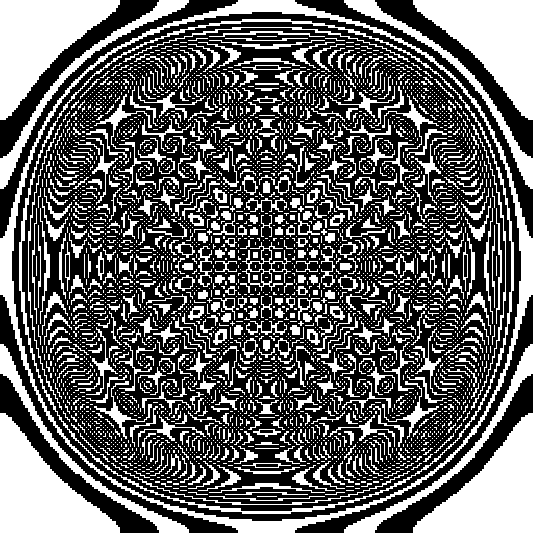
\includegraphics[width=0.6\textwidth]{parity_res_N256_t003.pdf}
\caption{The parity pattern at $t=0.03$ on a $256^2$ grid, $q=10$,
$832$ isotherms. An undersampled Fresnel zone plate: the central rings
are the real contour map of the peak, the surrounding lattice of small
concentric centres is moir\'e, replicas created where the local fringe
frequency matches a multiple of the sampling frequency, and the striped
sectors between them are digital planes. The figure is vector graphics;
zooming in shows the individual cells.}
\label{fig:zoneplate}
\end{figure}

\begin{figure}[ht]
\centering
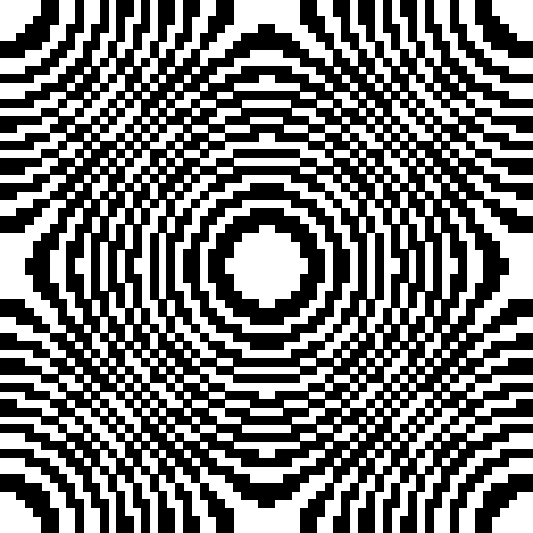
\includegraphics[width=0.3\textwidth]{parity_k2000.pdf}\hfill
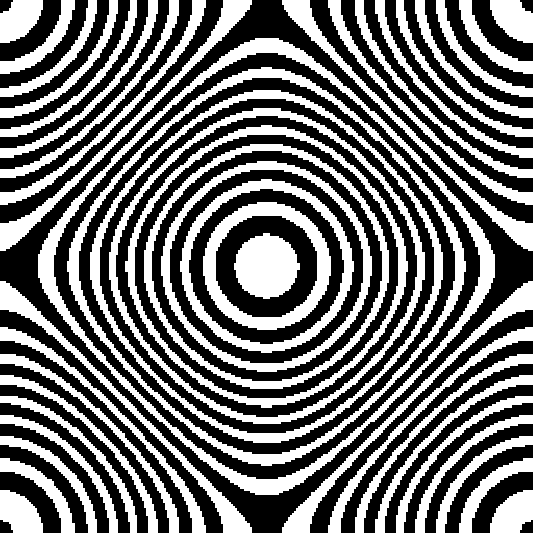
\includegraphics[width=0.3\textwidth]{parity_late_N256.pdf}
\caption{Left: $64\times64$ grid at $t=0.4$ ($q=10$). Right: the same
state on a $256\times256$ grid with the same quantum. The islands of the
left frame are replicated zone-plate centres; the right frame is the
contour map of the field, with its mirror images in the four corners
produced by the reflecting walls.}
\label{fig:res}
\end{figure}

\begin{table}[ht]
\centering
\begin{tabular}{@{}rrrrr@{}}
\toprule
$N$ & bands & perimeter$/N^2$ & $H_{2\times2}$ (bits) & components \\
\midrule
 64 & 34 & 1.082 & 3.93 & 905 \\
128 & 36 & 0.564 & 3.45 &  88 \\
256 & 37 & 0.287 & 2.61 &  92 \\
\bottomrule
\end{tabular}
\caption{Resolution test at $t=0.4$, $q=10$ fixed. Perimeter per cell
halves with each doubling, as a fixed set of smooth curves does; the
islands collapse into the real rings.}
\label{tab:res}
\end{table}

\section{What is not claimed, and what the lesson is}\label{sec:lesson}

The number of components of the pattern, and the number of local maxima
of $u$, are not monotone in general in two dimensions
\cite{Magnanini}; nor is the entropy of the value histogram of $u$. There
are no eddies: for $t>0$ the field is analytic with smooth nested
isotherms. The lesson is methodological. Perimeter, block
entropy and component counts of a thresholded simulation measure the
sampling as much as the dynamics; the phase-averaging identity
\eqref{eq:phase} is a diagnostic, since a phase-averaged perimeter
exceeding $q\TV_h$ is aliasing by Theorem~\ref{thm:grid}(3). Real
complexity requires the nonlinearity inside the dynamics: putting the
modulus into the update rule instead of the display gives Wolfram's
continuous cellular automata \cite[ch.~4]{NKS}, coupled map lattices in
the sense of \cite{Kaneko}, which do have localized structures; their
interaction with reflecting walls is the subject of a companion paper
\cite{MirrorWalls}.

\paragraph{A remark on functional information.} Wong et al.\
\cite{Wong2023} have proposed a law of increasing functional information:
the functional information of a system increases when many
configurations of the system undergo selection for one or more
functions. Functional information, in the sense of Szostak and Hazen
\cite{Szostak2003,Hazen2007}, is $I(E_x)=-\log_2F(E_x)$, where $F(E_x)$ is
the fraction of all configurations that perform a given function to
degree at least $E_x$; it is defined only relative to a function, and
the proposed law makes selection, not mere dynamics, the source of its
growth. Quantized diffusion is a clean example of why the restriction to a function
is necessary. The quantized heat frames have no function and undergo no
selection; every quantity intrinsic to the field, the band count, the
total variation, the gradient, decreases monotonically
(Theorems~\ref{thm:cont} and~\ref{thm:grid}); and yet the
function-free complexity proxies that are commonly read as evidence of
``ratcheting'' complexity, perimeter, block entropy, component count,
rise from zero to near their maxima before they fall. The rise is
produced entirely by the observer's choices of quantum and grid, and
Theorem~\ref{thm:entropy} shows that these choices can make the block
entropy anything between zero and its maximum. The random-phase
identity \eqref{eq:phase} is the diagnostic that separates the two
cases: a phase-averaged perimeter above $q\TV_h$ is sampling, not
structure. A system has to do more than produce pictures that look
complex before the question of selection can even be asked; in the
companion paper \cite{MirrorWalls} we take automata that do sustain
persistent localized structures and ask whether the walls of a box act
on them as a selecting environment.

\section*{Code}
All scripts, the figures and the source of this article are public at
\url{https://github.com/MiguelPerezI/heat-parity-ca}: \texttt{analyze.py}
reproduces the frames and the measures of Table~\ref{tab:res},
\texttt{restest.py} the resolution test, and \texttt{phase\_theorem.py}
checks Theorem~\ref{thm:grid} and produces Table~\ref{tab:phase}.

\begin{thebibliography}{99}
\bibitem{TernaryCube}
M.~E.~P\'erez Ibarra, J.~Flores Rodr\'iguez,
\emph{One case, not twenty-seven: the ternary cube as the index set for
boundary stencils of finite-difference schemes in any dimension},
arXiv preprint (2026). [Insert arXiv identifier.]
\bibitem{NKS}
S.~Wolfram, \emph{A New Kind of Science}, Wolfram Media, 2002.
\bibitem{Magnanini}
R.~Magnanini, \emph{An introduction to the study of critical points of
solutions of elliptic and parabolic equations}, arXiv:1604.00530.
\bibitem{Amidror}
I.~Amidror, \emph{The Theory of the Moir\'e Phenomenon}, 2nd ed.,
Springer, 2009.
\bibitem{Evans}
L.~C.~Evans, \emph{Partial Differential Equations}, 2nd ed., AMS, 2010.
\bibitem{Harten}
A.~Harten, \emph{High resolution schemes for hyperbolic conservation
laws}, J.\ Comput.\ Phys.\ 49 (1983) 357--393.
\bibitem{MOW}
O.~Martin, A.~Odlyzko, S.~Wolfram, \emph{Algebraic properties of cellular
automata}, Comm.\ Math.\ Phys.\ 93 (1984) 219--258.
\bibitem{Kaneko}
K.~Kaneko, \emph{Overview of coupled map lattices}, Chaos 2 (1992) 279--282.
\bibitem{Hologram}
Analysis on image recovery for digital Fresnel hologram with aliased
fringe generated from self-similarity of point spread function,
arXiv:1911.07997.
\bibitem{Wong2023}
M.~L.~Wong, C.~E.~Cleland, D.~Arend~Jr., S.~Bartlett, H.~J.~Cleaves~II,
H.~Demarest, A.~Prabhu, J.~I.~Lunine, R.~M.~Hazen, \emph{On the roles of
function and selection in evolving systems}, Proc.\ Natl.\ Acad.\ Sci.\
USA 120 (2023) e2310223120.
\bibitem{Szostak2003}
J.~W.~Szostak, \emph{Functional information: molecular messages}, Nature
423 (2003) 689.
\bibitem{Hazen2007}
R.~M.~Hazen, P.~L.~Griffin, J.~M.~Carothers, J.~W.~Szostak,
\emph{Functional information and the emergence of biocomplexity},
Proc.\ Natl.\ Acad.\ Sci.\ USA 104 (2007) 8574--8581.
\bibitem{MirrorWalls}
M.~E.~P\'erez Ibarra, J.~Flores Rodr\'iguez,
\emph{Reflecting walls are self-collisions: localized structures of
cellular automata in a mirror box}, in preparation (2026).
\end{thebibliography}

\end{document}
